\chapter{Examples}
\label{ch:examples}
\label{ch:catalog}

\section{Ensemble-based CPS}  

\subsection{Overview}
%\STATUS{ready for review}
An Ensemble-Based Cyber-Physical System (EBCPS) is an emergent system\uidx{System} that is distributed\uidx{Distributed}, decentralized, dynamic, self-adaptive and scalable. It consists of autonomous components\uidx{Component} and forms ensembles of them depending on the context in the aim of achieving determined goals (i.e. organizing\uidx{Organization} and decision-making). More specifically, the composition\uidx{Compositionality} of components changes according to the fact of having the components appear and disappear dynamically, in addition to the unexpected changes in the environment and new requirements. There are many applications in different domains such as Traffic and Transport, Robotics, and Clouds. For instance, an ensemble of vehicle planning for optimal route with considering the road and traffic conditions. 

The interest of building such systems\uidx{System} was reflected in many European projects such as ASCENS\footnote{\url{http://www.ascens-ist.eu/}}, ALLOW Ensembles\footnote{\url{http://www.allow-ensembles.eu/}} and FoCAS \footnote{\url{http://www.focas.eu/}}, which are FP7 projects. ASCENS is oriented towards design and verification, while ALLOW Ensembles is more oriented towards performance. More specifically, ASCENS targets formalizing and modeling ensembles of autonomic-service components (SCs) that depend on knowledge units (K). It considers also the expression of self-adaption and provides tools and use cases. ALLOW Ensembles focuses on developing algorithms that improve ensembles utility and system dependability. Both previous projects are involved in FoCAS, which is a platform for communities that care about developing Collective Adaptive Systems (CAS\' s).

As part from ASCENS project, a formalism language was introduced to express the ensembles called Service Component Ensemble Language (SCEL) Figure~\ref{fig:Service_Component}. The language allows to define Knowledge, Behaviors\uidx{Behavioural}, Aggregations, and Policies. It allows the developer to define  interfaces with attributes or knowledge for Service Components (SCs) and their behavior using processes\uidx{Process}. Also, the developer can define the Service Component Ensembles (SCEs) and the conditions or policies to form them. The ensembles are responsible for exchanging knowledge between the components. Each ensemble evaluates the constraints\uidx{Constraint} over the interface attributes of the involved components. The support of context-awareness comes from using attributes in the constraint evaluation\uidx{Constraint} of forming ensembles.  
\begin{figure}[!htb]
\centering
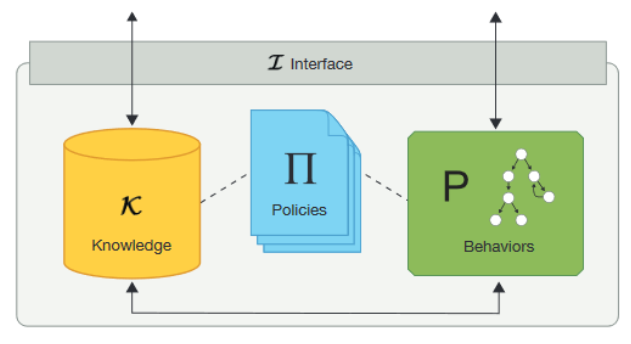
\includegraphics[scale=0.44]{figures/ServiceComponent.PNG}
\caption{Service Component}
\label{fig:Service_Component}
\end{figure}

Furthermore, ASCENS provides many tools for modeling (e.g. HELENA, KnowLang, DEECo) and for simulation (e.g. ARGoS, SPL, jDEECo Java, SimSOTA). Additionally, the concepts are presented in three use cases in different domains, which are: Clouds, Traffic and Transport, and Robotics.


\subsection{Dependable Emergent Ensembles of Components (DEECo)}
\uidx{Dependability}
To manifest the new concepts of EBCPS, the Department of Distributed and Dependable Systems (d3s: \url{http://d3s.mff.cuni.cz/}) at Charles University in Prague developed an EBCPS toolchain that is used as development environment which merges the concepts of emergent systems with the CPS parts\uidx{SystemPart} (i.e. physical, computational and network). More specifically, the parts that will be explained here are requirements, design, runtime, self-adaptation, analysis, composition and simulation. Moreover, there are many integrations and transformations\uidx{TransformationOperation} between the models.

\begin{figure}[!h]
\centering
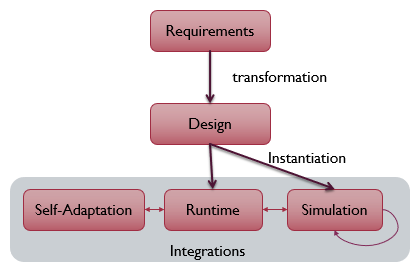
\includegraphics[scale=0.80]{figures/deeco_map.PNG}
\caption{Overview of the models provided by DEECo and their relations}
\label{fig:deeco_map}
\end{figure}

\subsubsection{Requirements}
Starting with modeling EBCPS requirements, Invariant Refinement Method (IRM) \cite{Keznikl:2013:DEC:2465449.2465457} (see  Figure~\ref{fig:irm}, which is developed in Epsilon, is used to represent the tree of invariants and assumptions for the system. The tree ends with leaves of two types: 1) processes\uidx{Process} which are part of a component\uidx{Component}, 2) or exchange knowledge between components\uidx{Component} which are ensembles. Simply put, the IRM allows to connect the requirements to the architecture entities directly. Later on, the developer can transform the IRM model to code which is Java for the current represented tool-chain under DEECo specification.

\begin{figure}[!htb]
\centering
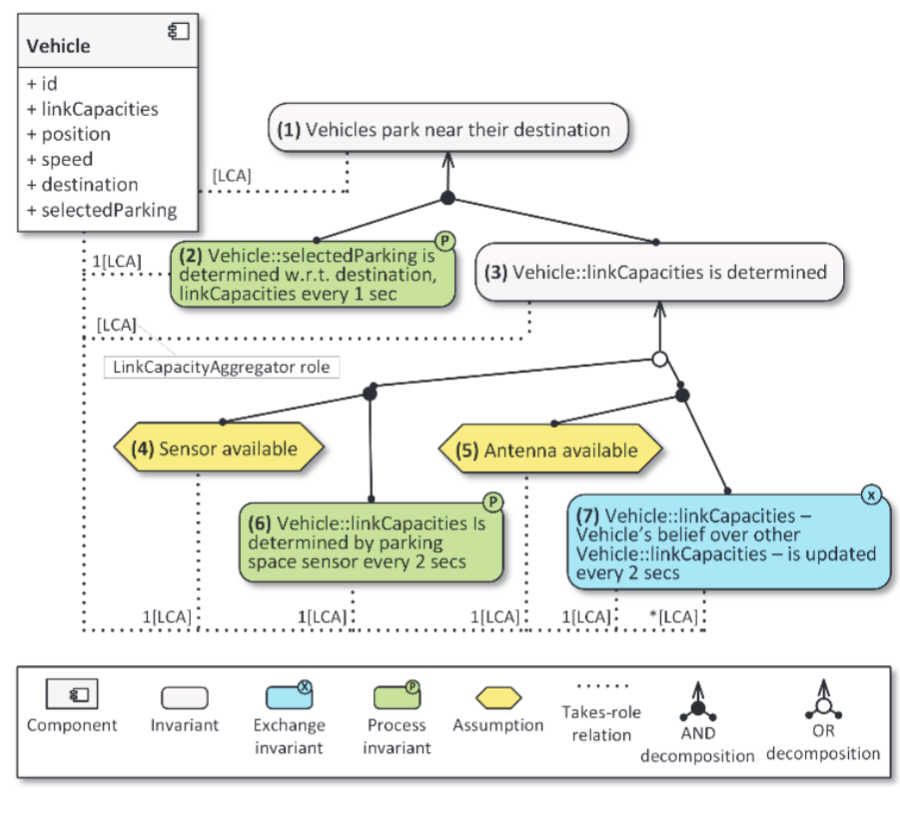
\includegraphics[scale=0.40]{figures/irm}
\caption{IRM tree for a smart parking senario}
\label{fig:irm}
\end{figure}

\subsubsection{Design and Runtime}

Regarding the design and runtime parts \cite{Bures:2013:DEC:2465449.2465462}\cite{AlAli:2014:DEC:2591062.2591140} , the team developed a runtime environment which is implemented in java and is known as jDEECo. The developer is able to design systems that respect the DEECo specification (i.e. SCEL specification), which is captured by specific Java annotations provided by jDEECo runtime Figure~\ref{fig:deeco_code}. More specifically, the designed system consists of roles\uidx{Role}, components\uidx{Component}, and ensembles\uidx{Ensemble}. Each role has a set of attributes, which represent the knowledge related to this specific role. Furthermore, each component is defined as a set of processes\uidx{Process} featuring (a) role(s) having by that the role knowledge besides its local knowledge. Having knowledge in the role allows for preserving the encapsulation of the components\uidx{Component} that features the role and provides a separation in concerns\uidx{Concern}. Hence, each ensemble forms depending on the context and perform knowledge exchange between different components with determined roles. 

\begin{figure}[!h]
\centering
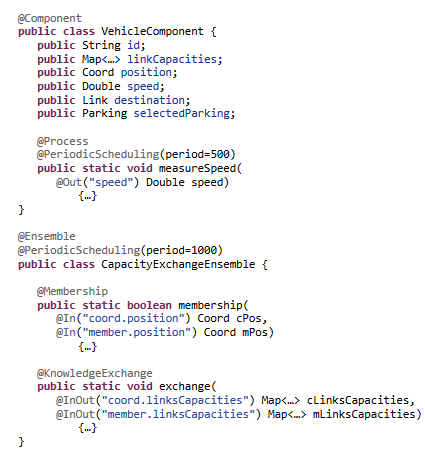
\includegraphics[scale=0.80]{figures/deeco_code}
\caption{Snippet of jDEECo code}
\label{fig:deeco_code}
\end{figure}

\begin{figure}[!h]
\centering
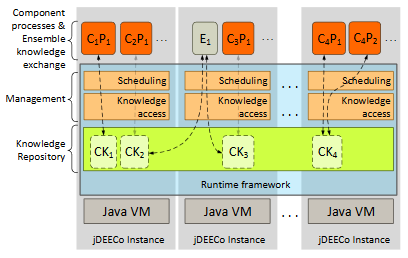
\includegraphics[scale=0.85]{figures/jdeeco}
\caption{jDEECo runtime framework architecture}
\label{fig:ros}
\end{figure}

 It is worth mentioning that there is another framework that integrates with jDEECo, which is called Intelligent Ensemble framework\footnote{\url{http://d3s.mff.cuni.cz/software/deeco/files/seams-2017.zip} or \url{http://dx.doi.org/10.4230/DARTS.3.1.6}} \cite{Krijt2017Intelligent}. It provides the developer with Ensemble Definition Language (EDL) that was developed using XText and XPand on Eclipse Modelling Framework. At runtime the formation of the ensemble is optimized by using Z3 SMT solver.  
 
\begin{figure}[!h]
\centering
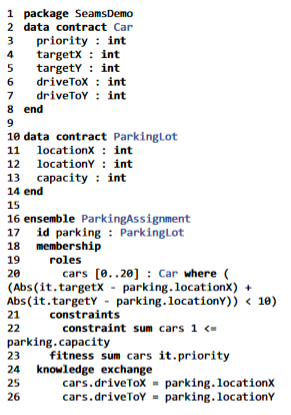
\includegraphics[scale=0.75]{figures/edlspec}
\caption{An example with an EDL specification}
\label{fig:ros}
\end{figure}


\begin{figure}[!h]
\centering
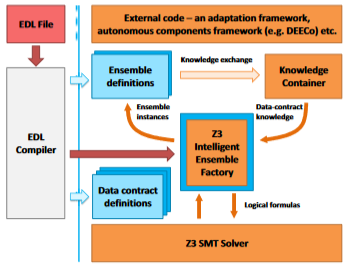
\includegraphics[scale=0.85]{figures/edl}
\caption{Framework high-level architecture that supports Ensemble Definition Language (EDL)}
\label{fig:ros}
\end{figure}

Not only is DEECo implemented in java, but also it is implemented in C++ \footnote{\url{http://d3s.mff.cuni.cz/projects/components_and_services/deeco/files/CDEECo.zip}} and Scala\footnote{\url{ http://github.com/d3scomp/tcof}}. Nevertheless, the model operations\uidx{ModelOperation} that we mentioned here (i.e. transformation\uidx{TransformationOperation} and integrations\uidx{IntegrationOperation}) are applied on jDEECo (i.e. java implementation).

 
\subsubsection{Self-Adaptation}
Self-adaptation is done in two methods. The first method is by transforming IRM tree to java code with annotations, then at runtime the annotations are processed by IRM-SA engine which uses SAT solver to make decisions between the different paths. The other method is by using modes and mode-switching annotations that are provided by DEECo. It is possible to associate a mode to a set of processes, thus when a mode-switch happens a different set of processes is activated.

There is a part that is presented as an extension of mode-switch transition logic, which are: 1) ordinary differential equation (ODE) to evaluate the inaccuracy\uidx{Accuracy} boundaries of physical attributes~\cite{10.1109/WICSA.2014.20}, 2) statistical testing to use prediction depending on trends of historical data~\cite{7516826}.

Another essential point that DEECo focuses on is forming ensembles and exchanging knowledge. DEECo manifests those concepts and allows for using conditions that are a representation of context to form ensembles. The conditions are refined by using a Z3 SMT Solver~\cite{Krijt2017Intelligent} and fitness, which filter out the less suitable compositions between all possible ones. Regarding exchanging knowledge between components\uidx{Component}, it could be determined by context constraints\uidx{Constraint} or by adding boundaries on gossip protocol that is responsible of spreading information~\cite{Bures2014}. Furthermore, DEECo allows a hierarchical composition for ensembles~\cite{Bures:2015:TIE:2797433.2797450}\cite{Bures2016}.

\begin{figure}[!htb]
\centering
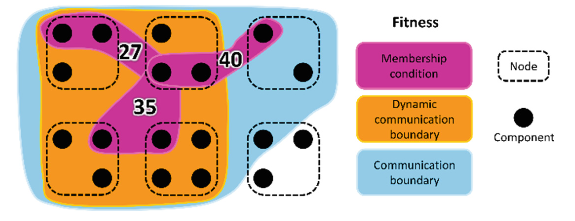
\includegraphics[scale=0.60]{figures/fitness}
\caption{Membership vs. boundary conditions in ensemble formation}
\label{fig:fitness}
\end{figure}

\subsubsection{Simulation}
Finally, the simulation part targets two domains for vehicles\cite{Kit:2015:AFE:2821357.2821374} and robots\cite{Matena:2016:MPT:2897053.2897065}. Concerning vehicles, jDEECo has an integration with MATSim which allows to simulate vehicles and OMNET++ which simulates the network delays. Regarding the robots case, jDEECo has an integration with ROS which simulates movements of robots. While ROS has in its turn an integration with OMNET++ to simulate network delays and with Stage to simulate sensors and actuators.

\begin{figure}[!htb]
\centering
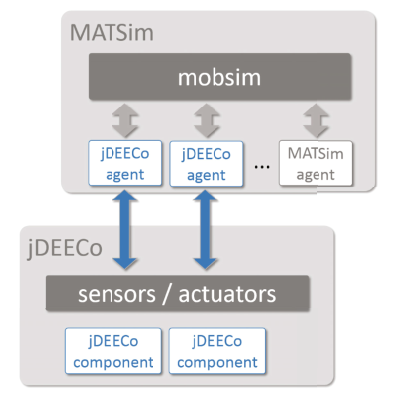
\includegraphics[scale=0.55]{figures/matsim}
\caption{jDEECo integration with MATSim}
\label{fig:matsim}
\end{figure}

\begin{figure}[!htb]
\centering
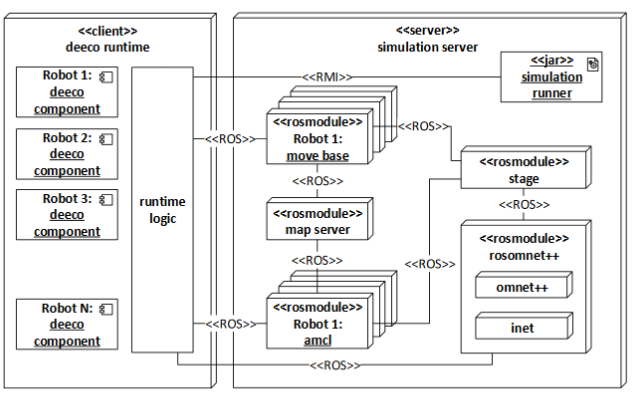
\includegraphics[scale=0.65]{figures/ros}
\caption{jDEECo integration with ROS}
\label{fig:ros}
\end{figure}


 To conclude, DEECo development environment provides a toolchain for modeling CPS system with an emergent behavior\uidx{BehaviouralCharacteristic} starting from requirement to runtime and simulation. To get the different views of system developmen,t many transformation and integration operations\uidx{IntegrationOperation} are involved which supports the idea of multi-paradigm modeling\uidx{Paradigm}. These are further presented in the developed ontology of DEECo briefly presented below.
 
 
 
\subsubsection{Applications}
%\STATUS{descriptions of presented use cases in different domains}
  Many applications were introduced using DEECo concepts, which are in Automotive, Robotics, Clouds and Industry domains. 
 
 The Automotive example \cite{Hoch2015emobi} is basically to present aspects of requirements, self-adaptation, networking, and simulation. The IRM tree represents finding a free parking and MATSim \footnote{\url{https://matsim.org}} simulates the traffic. The models involved in this example are IRM Model, DEECo Design time Model, DEECo Runtime Model, and MATSim. Furthermore, in  \cite{Kit2015empl}, the example presents road trains that use MANETs network and utilizes the knowledge exchange by using bounded gossiping \cite{10.1007/978-3-319-09970-5_23}.

\begin{figure}[!htb]
\centering
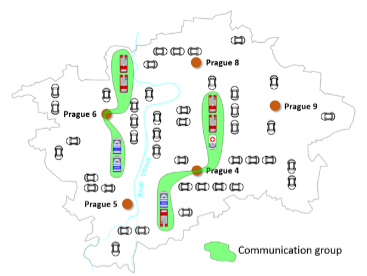
\includegraphics[scale=0.85]{figures/gossip}
\caption{Illustration of communication\uidx{Communication} groups; each is associated with an instance of SameDestination}
\label{fig:gossip}
\end{figure}

Also, a railroad emergency response service example includes trucks helping damaged trains (e.g. because of low fuel quality) \cite{modelsward17}. The service should take into account the performance and the balance in serving between different clients. In other words, repairing the trains should be fast, but also the trucks should consider the situation in case another farther train was damaged at the same time (i.e. not only going to the closest train). Here, the development starts with defining EDL Files, compiling them, and then generating the DEECo Design time Model. At runtime, the DEECo Runtime Model integrates with Z3 SMT Solver to optimize forming the ensembles.

\begin{figure}[!htb]
\centering
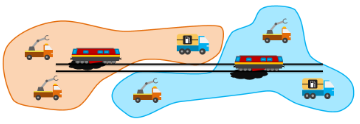
\includegraphics[scale=0.85]{figures/trains}
\caption{Example of two well-chosen emergency groups.}
\label{fig:trains}
\end{figure}

The FireFighter Coordination example is another example that represents the use of IRM-SA model and DEECo \cite{Gerostathopoulos:2017:SAC:3068423.2823345} \cite{GEROSTATHOPOULOS2016378}. The example describes groups of firefighters that have to operate using low-power nodes and without communication guarantees. The work presents self-adaptation using multi-layered architecture\uidx{Architecture}, which are: Meta-Adaptation Layer, Adaptation Layer,and Business System. Thus, the example involves IRM-SA model, Self-Adaptation Model, DEECo Runtime Model and DEECo Design time Model.
 
 Another example related to parking places but with edge cloud usage is presented in ~\cite{Bures:2018:PMS:3185768.3186306} Figure \ref{fig:parking}. The example describes vehicles that detect parking spots and informs other vehicles about it. The used simulation tool is Veins LTE, which is based on OMNeT++\footnote{\url{https://www.omnetpp.org}} (i.e. network simulator), INET\footnote{\url{https://inet.omnetpp.org}} and SimuLTE\footnote{\url{http://simulte.com}} (i.e. radio simulators), and SUMO\footnote{\url{http://sumo.dlr.de}} (i.e. road traffic simulator). The main concern\uidx{Concern} is performance model that is presented by Queueing Networks (QN), and it is planned to be integrated with DEECo. 
 
\begin{figure}[!htb]
\centering
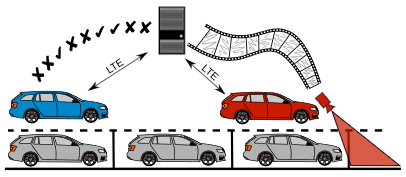
\includegraphics[scale=0.65]{figures/parking}
\caption{Scanning cars (on the right) are sending a photo stream to the edge cloud server reporting spot availability to the parking cars (on the left)}
\label{fig:parking}
\end{figure}
 
Regarding Clouds domain, the example concerns are performance and adaptation, and targets real-time guarantees for image processing application that runs on edge-cloud architecture [\cite{Hnetynka:2018:GLA:3241403.3241448}]. The work is in progress and it will involve Statistical Model with Self-Adaptation Model from the current models. 

As for predictability\uidx{Predictability} and adaptability\uidx{Adaptability}, the use case present cleaners that detect the need for charging or cleaning, and the active mode is determined statistically to avoid premature mode-switch \cite{bures2016stat}. This example involves the statistical mode-switching in Self-Adaptation Model, in addition to DEECo Design time Model and DEECo Runtime Model. The evaluation of statistical functions was done on STM32F4-DISCOVERY board. 
 
 \begin{figure}[!htb]
\centering
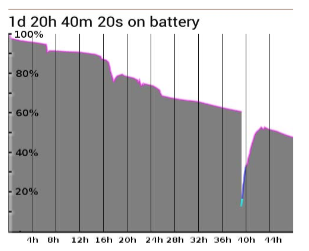
\includegraphics[scale=0.65]{figures/statistical}
\caption{Sample battery energy level during continuous discharge }
\label{fig:statistical}
\end{figure}

 
 Another case is Autonomous Cleaning  Robots  Coordination (ACRC) \cite{Matena2016Model} where robots have tasks of visiting and cleaning the offices. The problems that robots encounter here are imprecise localization, limited communication range, and latencies, which are solved by introducing self-healing in the self-adaptation logic. The testbed is done using ROS simulation for robots with camera (i.e. Stage) for navigation and IEEE 802.15.4 transceiver for communication (i.e. OMNet++). \footnote{\url{http://d3s.mff.cuni.cz/projects/components_and_services/deeco/files/seams-2016-artifact.zip}}
 
 \begin{figure}[!htb]
\centering
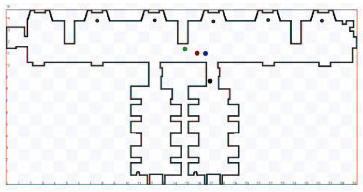
\includegraphics[scale=0.65]{figures/robots}
\caption{A visualization of the the area that cleaners should visit and clean}
\label{fig:robots}
\end{figure}

The scalability\uidx{Scalability} issue was targeted in an example about intelligent production line (IPL) \footnote{\url{https://github.com/d3scomp/scalable-reliability}} \cite{Matena2017enssca}. The example also aims at preserving the safety\uidx{Safety} conditions in the work place with taking into account the scalabe QoS grantees. To put it differently, the robots have safety zone and speed grantees, which change depending on the number of human and robots in the area. The used models are OMNeT++ and INET simulators with DEECo Design Model and DEECo Runtime Model.
\begin{figure}[!htb]
\centering
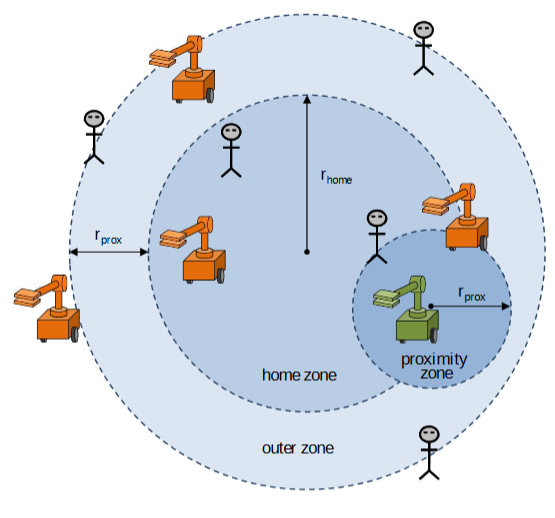
\includegraphics[scale=0.50]{figures/productionline}
\caption{Intelligent production line: home, proximity, and outer zones}
\label{fig:productionline}
\end{figure}

 The privacy and trust use case describes the exchange of the sensitive data between companies or inside the company itself \cite{Al-Ali:2018:MDT:3241403.3241450},\cite{10.1007/978-3-030-03424-5_12},\cite{alali2018usecases} (i.e. as part of Trust 4.0 project\footnote{\url{http://trust40.ipd.kit.edu/home/}}). More specifically, the system preserves information by preventing physical encounter between different teams, which is done through granting/denying access for the employees depending on the time table and existing people in the room \cite{10.1007/978-3-030-03424-5_12}. Another example is about production shifts, the foreman role has access only for employees' names in that shift. In case the system detects a possible delay of one of the employees, the system grants the foreman an access to name and phone number of a backup employee. Similarly, the confidentiality\uidx{Confidentiality} levels between companies depends on the context such as encountering incidents. These examples uses the basic concepts of DEECo (i.e. DEECo Design time Model and DEECo Runtime Model) in Scala \footnote{\url{https://www.scala-lang.org/}}. It involves fitness model in the lunch room example \cite{10.1007/978-3-030-03424-5_12}, and ValueStreamer \footnote{\url{https://www.valuestreamer.de/en/home/}} and PCM \footnote{\url{https://www.palladio-simulator.com/science/palladio_component_model/}} on industry 4.0 example.   
 
\begin{figure}[!htb]
\centering
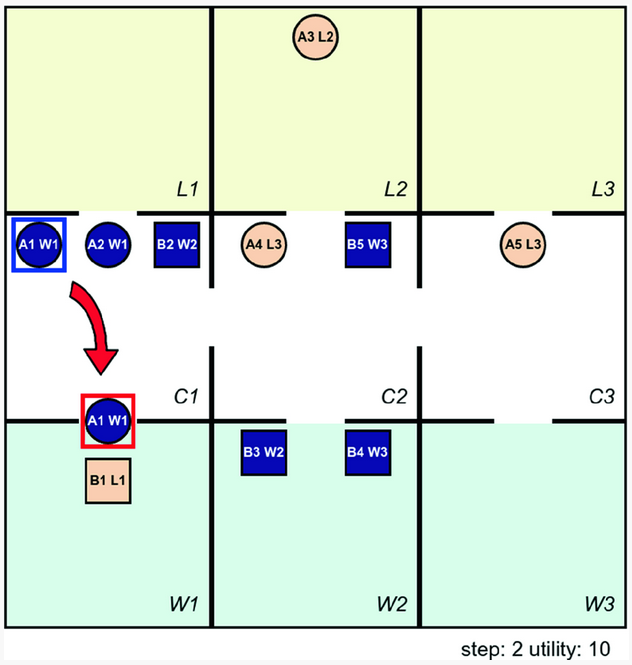
\includegraphics[scale=0.44]{figures/lunchroom}
\caption{Entry for the developer A1 to room W1 is rejected due to the presence of the developer B1}
\label{fig:lunchroom}
\end{figure}

  
 \begin{figure}[!htb]
\centering
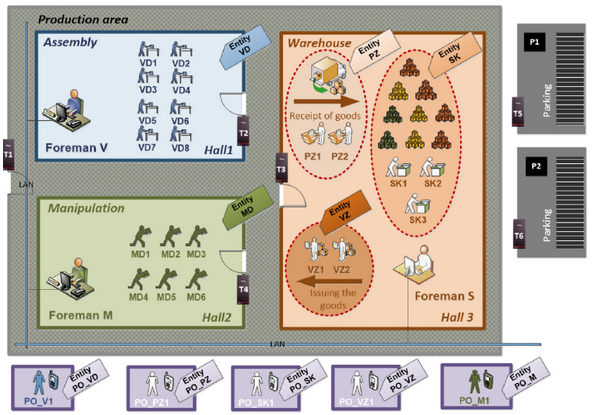
\includegraphics[scale=0.70]{figures/shifts}
\caption{The use case illustrates a production area, which has many halls. For each hall, there is a single foreman who manages the workers.}
\label{fig:shifts}
\end{figure}
 
\subsection{Ontology}
 The structure\uidx{StructureCharacteristic} of DEECo is described using the ontologies provided by MPM4CPS. This is done by instantiating its classes, so the created set of individuals represents DEECo.
 
 \subsubsection{CPS}
% \STATUS{ready for review}
In this part, the individuals represents the system domain and its parts\uidx{SystemPart}, in addition to the its requirements.
 \begin{itemize}
     \item ApplicationDomainsDS\uidx{ApplicationDomain}: BuildingAutomation, IntelligentTransport, RoboticForService, SmartManufacturing
     \item \uidxp{Architecture}: Generic Architecture
     \item SystemDC: 
        \subitem \uidx{SystemPart}: regarding the CommunicationProtocol, the short range communication\uidx{Communication} (P2P) is used in most of the use cases (e.g. MANET, gossip protocol, ...). 
        \subitem \uidx{Component}: entities which are modeled in CPS using DEECo are hardware/physical components. For instance, vehicle or cleaner are physical components with a need for representation of physical process dynamics (i.e. differential equations). Additionally, it is possible to model components\uidx{Component} in the environment such as human.
           
    \item QualityRequirementsDC
        \subitem \uidxp{Dependability}: \uidxp{Safety}, \uidxp{Availability}
        \subitem \uidxp{Interoperability}: \uidxp{Scalability}
        \subitem \uidxp{Predictability}: \uidxp{Accuracy}
        \subitem \uidxp{Reliability}: \uidxp{Robustness} 
        \subitem \uidxp{Security}: \uidxp{Confidentiality}
        \subitem \uidxp{Sustainability}: \uidxp{Adaptability}, \uidxp{Efficiency} (i.e. performance), \uidxp{Resilience} 
 \end{itemize}
 

 \subsubsection{MPM}
% \STATUS{ready for review}
  In this part, the individuals includes a DEECo megamodel\uidx{Megamodel} and its fragments\uidx{MegamodelFragment} defining all model operations\uidx{ModelOperation} supported by DEECo as outlined in Figure~\ref{fig:deeco_map} and Figure~\ref{fig:deeco_ontology}. Model operations\uidx{ModelOperation} are of different kinds such as transformation and integrations operations\uidx{IntegrationOperation}. The first model operation is the capture of requirements followed by a transformation operation\uidx{TransformationOperation} from the requirements model into a design model, then by an instantiation operation to create runtime model and simulation model. The runtime model integrates with the self-adaptation model Figure~\ref{fig:deeco_tools}.

\begin{figure}[!htb]
\centering
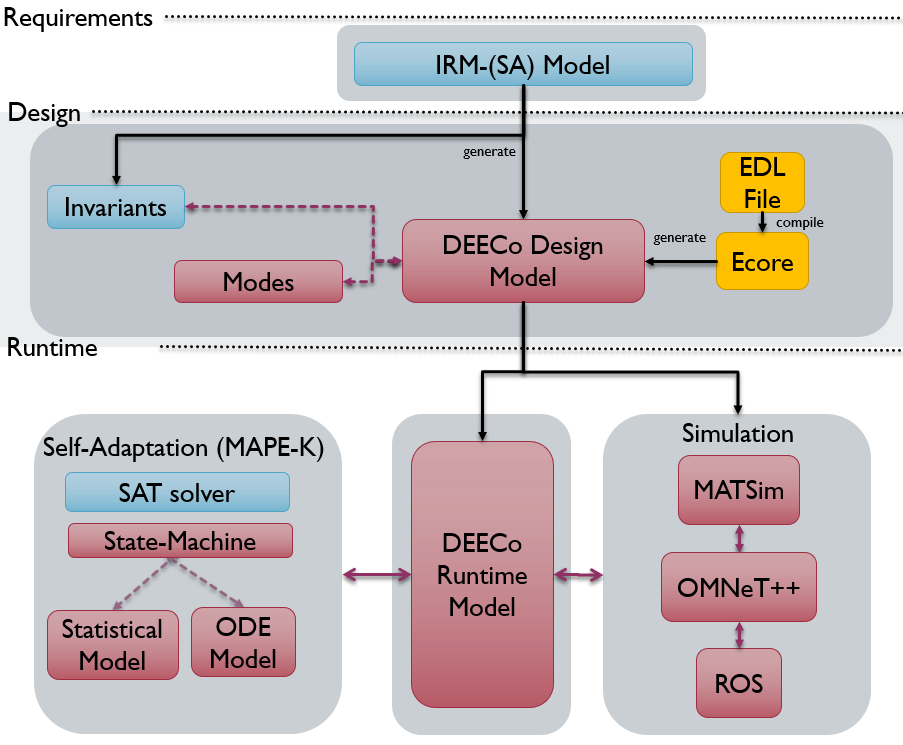
\includegraphics[scale=0.50]{figures/deeco_tools_adv.PNG}
\caption{Models and Tools Transformations and integrations}
\label{fig:deeco_tools}
\end{figure}

\begin{figure}[!h]
\centering
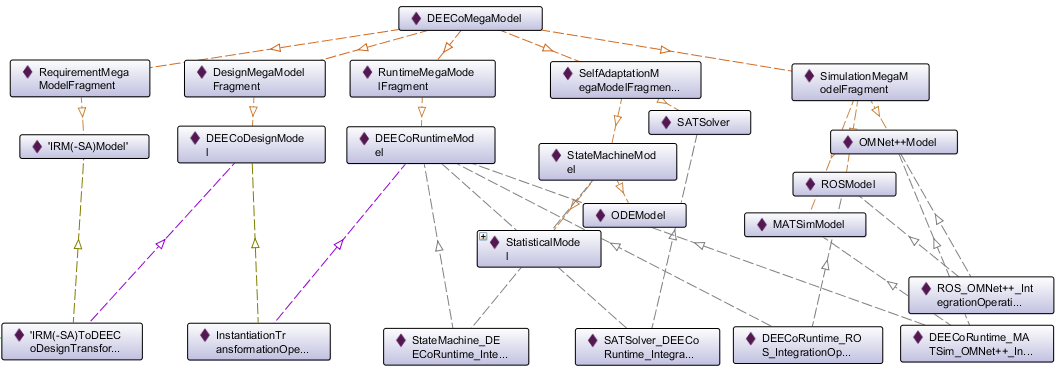
\includegraphics[scale=0.55]{figures/ontology.PNG}
\caption{The example of DEECo represented by OntoGraf using Protege}
\label{fig:deeco_ontology}
\end{figure}

\subsubsubsection{\textbf{Formalism, Models, and Tools}}

\begin{itemize}
    \item \uidxp{Formalism}
        \subitem \uidxp{AutomataBasedFormalism}: LTS (Labeled Transition System)
    \item Language
        \subitem \uidxp{FormalLanguage}: SCEL (Service Component Ensemble Language)
        \subitem \uidxp{ArchitecturalDescriptionLanguage}: DEECo realizes SCEL
        \subitem \uidxp{ModelingLanguage}: IRM, IRM-SA 
 %       \subitem ProgrammingLanguages: Java
 %       \subitem TransformationLanguages: Epsilon 
    \item Model
        \subitem MegaModel: DEECo (DEECo stands for Dependable Emergent Ensembles of Components)
        \subitem MegaModelFragment: \textit{mentioned below in details}
    \item ModelRelation: \textit{mentioned below in details}
    \item Tool
        \subitem ModelingTool: IRM-SA (Invariant Refinement Method - Self-Adaptation) developed in D3S Charles University in Prague, EclipseEpsilon
        \subitem RuntimeTool: jDEECo from Department of Distributed and Dependable Systems, Charles University in Prague
        \subitem SimulationTool: ROS from Open Source Robotics Foundation, OMNet++ from OpenSim Ltd,  MATSim from MATSim Community %, Stage from Richard Vaughan and contributors 1998-2011 Part of the Player Project
\end{itemize}


\subsubsubsection{\textbf{MegaModel Fragments / Models for DEECo}}
\begin{itemize}
    \item Requirements MegaModel Fragment\uidx{MegamodelFragment}
        \subitem Models: IRM Model 
    \item Design MegaModel Fragment
        \subitem Models: DEECo Design Model 
    \item Self-Adaptation MegaModel Fragment
        \subitem Models: IRM-SA Model, Mode-Switching Model 
    \item Runtime MegaModel Fragment
        \subitem Models: DEECo Runtime Model
    \item Simulation MegaModel Fragment
        \subitem Models: MATSim, ROS, OMNET++ %, Stage 
\end{itemize}


\subsubsubsection{\textbf{Tools / Model Operations for DEECo}}
\begin{itemize}
    \item Model Operation\uidx{ModelOperation}: Requirements Capturing Operation\uidx{CapturingOperation} - Modeling requirements refinements by Human
        \subitem Input: Human 
        \subitem Output Model(s): IRM-SA Model
        
    \item Model Operation\uidx{ModelOperation}: Requirements-Design Transformation Operation\uidx{TransformationOperation} - Capturing requirements refinements in design time
        \subitem Input Model(s): IRM-SA Model
        \subitem Output Model(s): DEECo Design Model 
        
   \item  Model Operation\uidx{ModelOperation}: Instantiation-Transformation Operation\uidx{TransformationOperation} - Instantiation of the DEECo components and ensembles 
        \subitem Input Model(s): DEECo Design Model
        \subitem Output Model(s): DEECo Runtime Model
        
   \item  Model Operation\uidx{ModelOperation}: Instantiation-Transformation Operation2\uidx{TransformationOperation} - Instantiation of the Simulation Model 
        \subitem Input Model(s): DEECo Design Model
        \subitem Output Model(s): ROS, MATSim , OMNet++ 

    \item Model Operation\uidx{ModelOperation}: Runtime-to-Vehicle Simulation Integration Operation\uidx{IntegrationOperation} - System Design Validation
        \subitem Input Model(s): DEECo Runtime Model
        \subitem Output Model(s): MATSim , OMNet++ 
        
    \item Model Operation\uidx{ModelOperation}: Runtime-to-Robot Simulation Integration Operation\uidx{IntegrationOperation} - System Design Validation
        \subitem Input Model(s): DEECo Runtime Model
        \subitem Output Model(s): ROS 
        
    \item Model Operation\uidx{ModelOperation}: Simulation-to-Simulation Integration Operation\uidx{IntegrationOperation} - System Design Validation
        \subitem Input Model(s): ROS
        \subitem Output Model(s): OMNet++ %, Stage 
    
\end{itemize}

 \subsubsubsection{\textbf{Development Process}}

The development process\uidx{Process} starts with capturing requirements operation in which a human is responsible of defining the IRM-SA model. Afterwards, the IRM tree is transformed to DEECo Design Model, which its instantiation are DEECo Runtime Model and Simulation Models. 

The DEECo Runtime Model is integrated with self-Adaptation model. It is possible also to define modes and their transitions in DEECo Design time model. Hence, the logic over transitions are extensible with ODE or statistical reasoning. Similarly, it is possible to define in the DEECo Design Model formation of ensembles by using gossiping boundary and fitness. The boundary defines limits on gossiping protocol and the fitness evaluates the history of forming ensembles and select the best fitting group of components that are involved to form the ensemble.

Finally, DEECo Runtime Model is also integrated with simulation models. For more information, please check the following links:
\begin{itemize}
    \item DEECO website: \url{http://d3s.mff.cuni.cz/software/deeco/}
    \item jDEECo: https://github.com/d3scomp/JDEECo/tree/simulation
    \item IRM: \url{http://d3s.mff.cuni.cz/software/irm/}
    \item Modes: \url{https://github.com/d3scomp/JDEECo/tree/master/jdeeco-modes}
    \item Statistical Operations: \url{https://github.com/d3scomp/TimeSeriesStatistics}
    \item OMNet++: \url{http://d3s.mff.cuni.cz/projects/components_and_services/deeco/files/jDEECo-OMNeT.zip}
    \item MATSim: \url{http://d3s.mff.cuni.cz/projects/components_and_services/deeco/files/jDEECo-MATSim.zip}
    \item ROS: \url{http://d3s.mff.cuni.cz/projects/components_and_services/deeco/files/seams-2016-artifact.zip}
    \item Intelligent Ensemble framework: \url{http://d3s.mff.cuni.cz/software/deeco/files/seams-2017.zip}
\end{itemize}


\subsubsection{MPM4CPS}
In this part, the views\uidx{View} and viewpoints\uidx{ViewPoint} for this system are described as following:

\begin{itemize}
 
    \item View\uidx{View}: Requirement Designer
    \item ViewPoint\uidx{ViewPoint}: The concerns\uidx{Concern} in this viewpoint is related to resilience\uidx{Resilience}, and involves both roles and ensembles in the system. The designer determines the environmental assumptions to each choice to ensure preserving the required invariants. That makes this viewpoint related to the cyber part of the system\uidx{SystemPart} (i.e. software).
    
    \item View\uidx{View}: Component Designer
    \item ViewPoint\uidx{ViewPoint}: The concerns\uidx{Concern} in this viewpoint is related to performances, accuracy\uidx{Accuracy}, robustness\uidx{Robustness} and self-adaptation. It involves designing roles\uidx{Role}, processes\uidx{Process} and modes\uidx{Mode}, in addition to relations\uidx{Relation} between processes and the assumptions from requirement phase. Also, components contain controllers, sensors, and actuators, which means that this viewpoint is related to physical and cyber parts of the system\uidx{SystemPart}.   
    
    \item View\uidx{View}: Ensemble Designer
    \item ViewPoint\uidx{ViewPoint}: The concerns in this viewpoint are related to knowledge exchange, security\uidx{Security}, optimization, scalability\uidx{Scalability} and performances. The designer should determine the roles\uidx{Role} involved in ensembles, the context constraints and what information to exchange. Additionally, the designer can optimize forming the ensembles by using fitting function and defining a boundary over gossip protocol. The design of ensembles could be also associated to system requirements as it is mentioned in the Requirement Designer view. This makes this viewpoint related to network and cyber (i.e. software) parts of the system\uidx{SystemPart}.
    
\end{itemize}
